\documentclass[11pt]{article}
\usepackage{amsmath}
\usepackage{amssymb}
\usepackage{pgfplots}

\begin{document}

LaTex document for LAFF class: notes
\\
\\
Homework 1.3.3.1
\\
\\$($
$\begin{bmatrix}
{-1} \\
{2}
\end{bmatrix}
+
\begin{bmatrix}
{-1}\\
{2}
\end{bmatrix}
$)$
+
\begin{bmatrix}
{-1}\\
{2}
\end{bmatrix}
$)$
=
\begin{bmatrix}
{-3}\\
{ 6}
\end{bmatrix}
$
\\
\\
\\
Homework 1.3.3.2
\\
\\
3 
x
$
\begin{bmatrix}
{-1}\\
{2}
\end{bmatrix}
=
\begin{bmatrix}
-{3}\\
{ 6}
\end{bmatrix}
$
\\
\\
\\
Homework 1.3.3.3\\
\\
\begin{tikzpicture}
\begin{axis}[
	xmin=-2, xmax=2,
	ymin=-2, ymax=2,
	axis lines = center,
	axis on top=true,
	domain=0:1,
]
\addplot [mark=none,draw=blue,ultra thick]{x};
\end{axis}
\end{tikzpicture}
\\
\\Which vector equals: \\
\\
\\
\\
\newpage
i)2a\\
\\
d
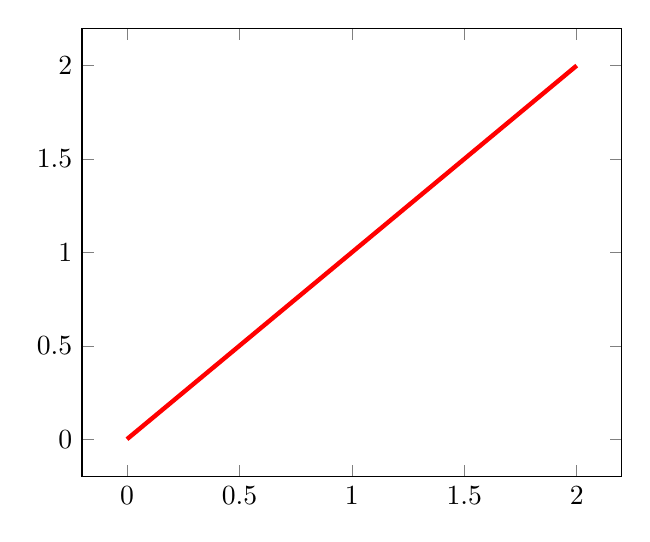
\begin{tikzpicture}
\begin{axis}

	\addplot+[mark=none,draw=red,ultra thick] coordinates
		{(0,0)(2,2)};
\end{axis}
\end{tikzpicture}
\\
\\
\\
ii)(1/2)a\\
b
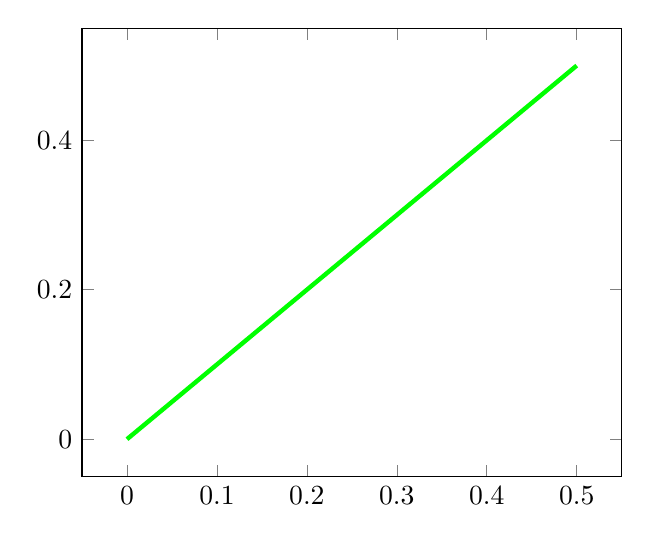
\begin{tikzpicture}
\begin{axis}

	\addplot+[mark=none,draw=green,ultra thick] coordinates
		{(0,0)(0.5,0.5)};
\end{axis}
\end{tikzpicture}
\\
\\
\newpage
iii)-(1/2)a\\
c
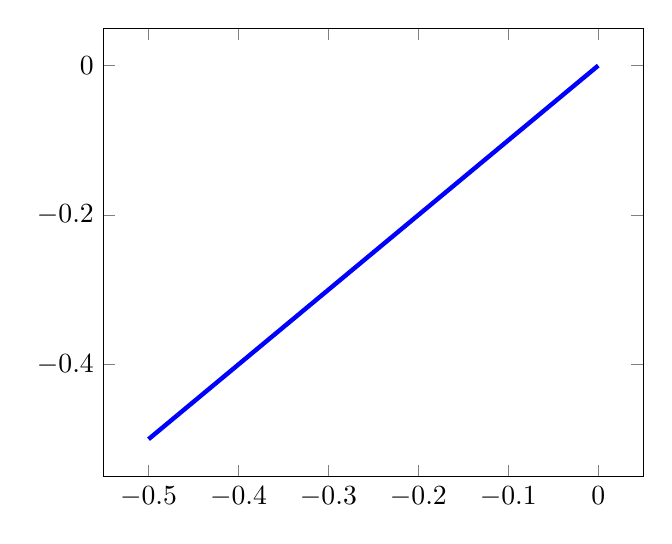
\begin{tikzpicture}
\begin{axis}

	\addplot+[mark=none,draw=blue,ultra thick] coordinates
		{(-0.5,-0.5)(0,0)};
\end{axis}
\end{tikzpicture}
\\

\end{document}

